\documentclass[12pt, a4paper]{article}
% \setlength{\parindent}{0pt} 
% \setlength{\parskip}{1em}
\usepackage[utf8]{inputenc}
\usepackage[polish]{babel}
\addto\captionspolish{
  \renewcommand{\figurename}{Wykres}
}
\usepackage{caption}
\captionsetup[figure]{font={small,bf},labelfont=bf}
\captionsetup[table]{font={small,bf},labelfont=bf}
\usepackage[T1]{fontenc}
\usepackage[colorlinks=true, linkcolor=black, urlcolor=blue]{hyperref}
\usepackage{pdfpages}
\usepackage[titletoc,title]{appendix}
\usepackage[nohyperlinks]{acronym}
\usepackage{listings}
\lstdefinestyle{verbatimStyle}{
    basicstyle=\ttfamily,
    columns=fullflexible,
    breaklines=true,
    breakatwhitespace=true,
    escapeinside={(*@}{@*)}, % opcjonalnie, aby umożliwić umieszczanie innych komend LaTeXa w środku
}

\title{Wykorzystanie analizy big data na statystykach meczów tenisowych w celu poprawy przygotowania i wyników zawodnika}
\author{Paweł Safuryn}
\date{2023}


\begin{document}


\includepdf[linktodoc=true,pages=-]{praca_koncowa_strona_tytulowa_BD.pdf}



\tableofcontents
\newpage

\section*{Akronimy}
\addcontentsline{toc}{section}{Akronimy}
\begin{acronym}
\acro{API}{Application Programming Interface}
\acro{ATP}{Association of Tennis Professionals}
\acro{AWS}{Amazon Web Services}
\acro{CLI}{Command-line Interface}
\acro{EMR}{Elastic MapReduce}
\acro{ETL}{Extract, Transform, Load}
\acro{GUI}{Graphical User Interface}
\acro{ID}{Identification}
\acro{MiB}{Mebibajt (1 048 576 bajtów)}
\acro{ML}{Machine Learning}
\acro{WTA}{Women's Tennis Association}
\end{acronym}



\section{Wstęp}
Tenis ziemny jest sportem indywidualnym, w którym nawet najmniejsza różnica może decydować o zwycięstwie. Zdarza się, że zwycięzca meczu zdobywa mniej punktów niż przegrany. Możliwe jest to dzięki (nieco skomplikowanym) zasadom punktacji. W tenisie, podobnie jak w innych sportach, analityka danych może właśnie stanowić tę kluczową różnicę między zwycięstwem a porażką. Jednak, w przeciwieństwie do innych sportów (np. baseball, piłka nożna), analityka danych w tenisie jest tematem stosunkowo nowym i nierozwiniętym pomimo ogromnej ilości szczegółowych danych zbieranych podczas meczów profesjonalnych rozgrywek. Powodem może być to, że tenis jest dosyć drogim sportem indywidualnym (w zespole zawodnika zazwyczaj nie ma miejsca dla analityka danych) o tradycyjnym wizerunku, który skutecznie zniechęca organizacje tenisowe, trenerów i zawodników do jakichkolwiek zmian. Niemniej jednak danych jest dużo i potencjał do zmian istnieje. Do takich danych należą między innymi:
\begin{itemize}
    \item Wysokopoziomowe statystyki meczów, np. wynik (sety, gemy), liczba asów, podwójnych błędów, wygranych punktów po pierwszym i drugim serwisie, itd.
    \item Szczegółowe statystyki meczów, np. historia meczu punkt po punkcie.
    \item Nagrania wideo meczów tenisowych, które mogą zostać poddane analizie, np. śledzenie piłki i ruchu zawodników.
    \item Informacje z systemu Hawk-Eye (elektroniczny system umożliwiający rozstrzygnięcie kontrowersyjnych punktów), np. trajektoria piłki, prędkość piłki, rotacja piłki itd.
    \item Warunki fizyczne zawodników.
\end{itemize}
Niestety większość szczegółowych danych nie była i nadal nie jest dostępna publicznie. Do tej pory, dostęp do tych danych był dostępny za opłatą i tylko dla profesjonalnych zawodników. Poza samym dostępem do danych dochodzą koszty zatrudnienia analityka danych, co sprawia, że zaawansowana analiza danych pozostaje zarezerwowana głównie dla najbardziej zamożnych graczy. Dopiero w drugiej połowie roku 2023 zaczęły pojawiać się głosy, że organizacje tenisowe (np. ATP) otwierają się na udostępnianie (w ograniczonym zakresie) danych z systemów takich jak Hawk-Eye \cite{the_telegraph}.

Główną korzyścią analizy tenisowych danych jest to, że pozwala ona zauważyć powtarzalne wzorce, których człowiek nie jest w stanie dostrzec podczas oglądania meczów na żywo lub na nagraniu wideo. Pozwala to zawodnikom (i ich trenerom) na, między innymi:
\begin{itemize}
    \item Zrozumienie słabych stron zawodnika i przygotowanie odpowiedniego treningu.
    \item Zrozumienie słabych i mocnych stron przeciwnika i opracowanie odpowiedniej taktyki na mecz.
    \item Odpowiednie planowanie startów turniejowych i przerw między turniejami.
\end{itemize}
Ponadto szczegółowa analiza danych może pomóc narodowym organizacjom tenisowym w identyfikowaniu młodych talentów i efektywnym rozdysponowywaniu środków na ich rozwój.

\subsection{Cel i zakres pracy}
Celem pracy jest, jak sugeruje tytuł (,,Wykorzystanie analizy big data na statystykach meczów tenisowych w celu poprawy przygotowania i wyników zawodnika''), zbadanie potencjału analizy ogólnodostępnych statystyk meczowych w celu poprawy przygotowania i wyników zawodnika. Ze względu na trudności z pozyskaniem szczegółowych danych (opisane wcześniej) źródłem są surowe dane (wysokopoziomowe statystyki meczów, rankingi i informacje o zawodnikach) zebrane przez tenisowego pasjonata \cite{tennis_atp, tennis_wta}. Zbieranie tych danych opisane jest w sekcji \ref{sec:obtain_raw_data}. Używając tych danych, praca skupia się na:
\begin{itemize}
    \item Rozpoznaniu najlepszych i najgorszych nawierzchni (kort twardy, kort ziemny, trawa, dywan) dla tenisisty.
    \item Analizie jakości serwisu na różnych poziomach rankingu.
    \item Analizie wyników zawodników różnych narodowości w zależności od poziomu zmęczenia.
    \item Analizie jakości i skuteczności pierwszego serwisu w zależności od wzrostu zawodnika.
\end{itemize}
Skutecznie przeprowadzone powyższe analizy mogą pomóc zawodnikom, trenerom i organizacjom tenisowym lepiej planować ich pracę i osiągać lepsze wyniki.

Do przetwarzania i analizy tenisowych zbiorów danych wykorzystane zostały metody, narzędzia i aplikacje do przetwarzania dużych zbirów danych (\textit{big data}). Opisane są one w sekcji \ref{sec:aws_architecture}. Ważnym celem pracy było także zastosowanie kontroli wersji (Git) do konfiguracji i skryptów związanych z całym procesem przetwarzania i analizy danych. Dlatego, gdzie było to możliwe i praktyczne, użycie GUI zostało ograniczone i zamiast tego zastosowane zostały skrypty w Bashu i AWS CLI. Cały kod (włącznie z kodem \LaTeX użytym do napisania tej pracy) dostępny jest na moim repozytorium \href{https://github.com/safurynp/pw-big-data-final-project}{pw-big-data-final-project} na GitHubie.




% Proces Data Engineering/Science można podzielić w ogólności na kroki:
% 1. Zbieranie surowych danych
% 2. Przetwarzanie danych
% 3. Eksploracja danych
% 4. Czyszczenie danych
% 5. Modelowanie (opcjonalne)
% 6. Produkt oparty na danych (czyste dane, analiza, wyniki itp.)
% 7. Komunikacja wyników

\section{Ustawienie środowiska}
\subsection{AWS Academy Learner Lab i AWS CLI}
Projekt wykonywany jest z użyciem AWS Academy Learner Lab [61569] i AWS CLI version 2. AWS CLI jest konfigurowane poprzez skopiowanie ustawień AWS Academy Learner Lab (dostępnych pod przyciskiem ,,AWS Details'') do pliku:
\begin{verbatim}
~/.aws/credentials
\end{verbatim}
AWS Academy Learner Lab generuje tymczasowe dane uwierzytelniające do AWS CLI za każdym razem, gdy jest uruchomiony, co powoduje, że plik \verb|~/.aws/credentials| musi być aktualizowany.

% Add info about ~/.aws/config - default region

% TODO: check LabRole ARN for CLI - https://us-east-1.console.aws.amazon.com/iam/home?region=us-east-1#/roles/details/LabRole?section=permissions

Opis architektury Big Data i indywidualnych technologii AWS wykorzystanych podczas projektu znajduje się w sekcji \ref{sec:aws_architecture}.

\subsection{Narzędzia używane lokalnie}
Poniżej znajduje się lista głównych narzędzi używanych lokalnie podczas projektu:
\begin{itemize}
    \item Python (wersja 3.9) --- główny język programowania używany do przetwarzania i analizy danych.
    \item Bash --- używany do automatyzacji zadań, głównie tych wykorzystujących AWS CLI.
    \item MacTeX i \LaTeX --- używane do napisania tej pracy końcowej.
    \item GitHub i Git --- kontrola wersji. Cały kod dostępny na repozytorium \href{https://github.com/safurynp/pw-big-data-final-project}{pw-big-data-final-project}.
    \item Miniconda --- zarządzanie środowiskiem wirtualnym oraz bibliotekami programistycznymi (np. do Pythona). Środowisko może być załadowane używając:
\begin{verbatim}
conda env create -f environment.yml
conda activate big-data-env
\end{verbatim}

\end{itemize}

\section{Architektura Big Data w AWS} \label{sec:aws_architecture}
Wykres \ref{fig:aws_architecture} przedstawia ogólny zarys architektury Big Data w AWS użytej w projekcie.
\begin{figure}[h]
    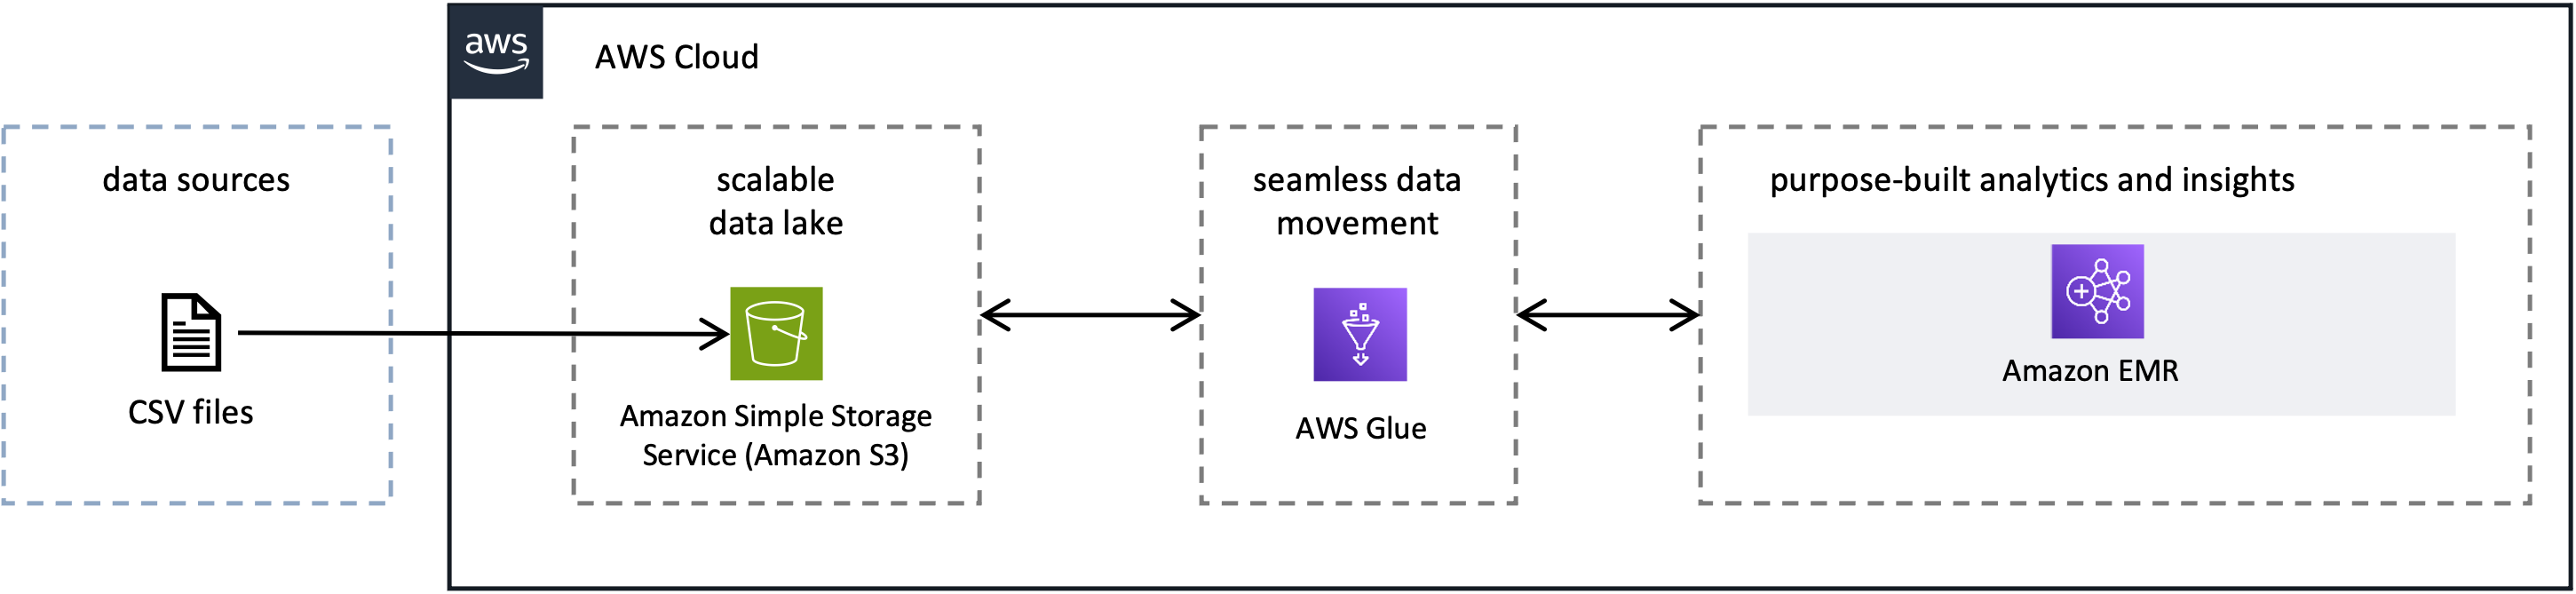
\includegraphics[width=\textwidth]{figures/aws_architecture.png}
    \caption{Architektura Big Data w AWS.}
    \label{fig:aws_architecture}
\end{figure}

Architektura ta składa się z następujących elementów:
\begin{enumerate}
    \item \textbf{Źródła danych}: Surowe dane w formacie plików CSV.
    \item \textbf{Skalowalny magazyn danych typu data lake}: 
    \begin{itemize}
        \item Amazon Single Storage Service (Amazon S3) używany do przechowywania surowych danych (bucket ,,tennis-stats-data'') oraz przetworzonych danych (bucket ,,processed-tennis-stats-data'').
        \item AWS Glue Crawler używany do automatycznego aktualizowania metadanych w katalogu danych.
        \item AWS Glue Data Catalog --- katalog danych używany do przechowywania metadanych o danych w Amazon S3.
    \end{itemize}
    \item \textbf{Zarządzanie przepływem danycb}: AWS Glue używany do eksploracji i przetwarzania danych za pomocą Notebooków AWS Glue i PySparka (Python API do Apache Spark).
    \item \textbf{Analityka i wizualizacja danych}:  Amazon EMR Notebook używany do analizy danych i tworzenia wykresów. Notebook używał PySparka i był uruchamiany na wcześniej przygotowanym klastrze Amazon EMR.
    % \item AWS QuickSight używany do wizualizacji danych i tworzenia dashboardów.
    \item \textbf{Logi}: Amazon CloudWatch używany do sprawdzania logów z Crawlera i procesów ETL w AWS Glue i klastrów Amazon EMR.

\end{enumerate}

% Moze:
% 1. Jakis Pipeline zeby ladowal automatycznie dane z repo Jeffa do S3 bucketow
%  - moze sprawdzac regularnie czy jest nowy commit i wtedy aktualizowac wszystkie dane
% 2. Zrob jakies konrketne trasnformacje na tych danych (oczyszczanie, itd.)
% 3. Wizualizacje i analityka

\section{Zbieranie danych}
\subsection{Pozyskanie surowych danych} \label{sec:obtain_raw_data}
Surowe tenisowe dane pozyskane są z dwóch repozytoriów na GitHubie Jeffa Sackmanna.
\begin{itemize}
    \item Dla profesjonalnego tenisa męskiego (ATP) \cite{tennis_atp}.
    \item Dla profesjonalnego tenisa żeńskiego (WTA) \cite{tennis_wta}.
\end{itemize}
Dane zostały pozyskane przez autora najprawdopodobniej (bazując na opisie repozytoriów) poprzez ekstrakcję danych (\textit{web scraping}) z Wikidata i oficjalnych stron organizacji ATP i WTA. Dane są dostępne w formacie CSV. Dane dla ATP i WTA mają ten sam format i zawierają:
\begin{itemize}
    \item Statystyki z singlowych meczów tenisowych z głównego cyklu turniejów ATP i WTA (np. Wielkie Szlemy, ATP/WTA 1000). Dostępne są dla każdego roku od 1968 (początek ery Open) do 2023. Statystyki dla każdego roku są zawarte w osobnym pliku CSV.
    \item Statystyki z singlowych meczów tenisowych z etapów eliminacji oraz z niższych rangą turniejów ATP i WTA (np. Challengers, Futures). Te dostępne są od lat 1968/1978/1991 (w zależności od rodzaju turnieju) do 2023. Statystyki dla każdego roku są zawarte w osobnym pliku CSV.
    \item Lista graczy tenisa ziemnego, którzy grali w profesjonalnym turnieju ATP lub WTA wraz z podstawowymi informacjami na ich temat.
    \item Informacje o profesjonalnym rankingu ATP i WTA (aktualizowane co tydzień) od lat 70 do 2023. Statystyki dla każdej dekady i roku 2023 są zawarte w osobnym pliku CSV.
\end{itemize}
W sumie są to 262 pliki CSV o całkowitym rozmiarze 395,7 MiB. W sumie są to informacje o 1 581 121 meczach, 2 621 tygodniach rankingów, 64 675 zawodnikach i 65 607 zawodniczkach. Repozytoria Jeffa Sackmanna na GitHubie zawierają również statystyki z meczów deblowych i amatorskich, ale te zostały pominięte w tym projekcie. Bardziej szczegółowy opis surowych danych znajduje się w załączniku \ref{sec:raw_data_description}.

Te dane zostały wybrane z poniższych powodów:
\begin{itemize}
    \item Zawierają wystarczająco szczegółowe informacje, aby przeprowadzić sensowne tenisowe analizy.
    \item Dane są ogólnodostępne i darmowe. Autor danych wymaga jedynie, aby zostały odpowiednio zacytowane.
    \item Dane są w powszechnym formacie CSV, co ułatwia ich początkową interpretację i przetwarzanie. Jednocześnie nie są to dane oczyszczone i wymagają obróbki (co pozwala an demonstrację odpowiednich technik przetwarzania danych big data).
    \item Rozmiar danych (395,7 MiB) nie jest typowym przykładem big data (w dzisiejszych czasach są to zazwyczaj petabajty lub eksabajty danych), ale jest na tyle duży, że przetwarzanie ich lokalnie mogłoby być czasochłonne i problematyczne. Jednocześnie rozmiar danych jest na tyle mały, że ich obróbka i analiza w ramach AWS Academy Learner Lab ze studolarowym (\$100) budżetem jest możliwa.
\end{itemize}

Inne źródła tenisowych danych również były rozważane. Między innymi było to użycie oficjalnych API od organizacji tenisowych, jednak takie nie były dostępne. Innym pomysłem była automatyczna ekstrakcja danych (\textit{web scraping}) z użyciem istniejących skryptów \cite{atp_web_scraping}, jednak skrypty nie działały po niedawnym przeprojektowaniu strony ATP i ograniczenia czasowe nie pozwoliły na tworzenie ich od nowa. Alternatywą było również pozyskanie niedawno udostępnionych oficjalnych danych od ATP \cite{atp_iq} jednak były one dostępne tylko dla profesjonalnych graczy.



% Napisz ile jest w sumie meczów w bazie danych, ile graczy (i ile tygodnie w rankingu, dla kazdego tygodnia pelny ranking)



\subsection{Przesyłanie danych do chmury AWS}
Surowe pliki CSV opisane powyżej zostały przesłane do chmury AWS w krokach opisanych poniżej:
\begin{enumerate}
    \item Trzy pliki CSV posiadające problem z kodowaniem UTF-8 (opisane bardziej szczegółowo w sekcji \ref{sec:explore}) zostały ręcznie oczyszczone.
    \item Do przechowywania plików CSV stworzony został bucket S3 o nazwie ,,tennis-stats-data'' z użyciem AWS CLI --- skrypt:
\begin{verbatim}
aws_cli/create_s3_raw_data.sh
\end{verbatim}
    \item Pliki CSV zostały przesłane do bucketu S3 z użyciem AWS CLI --- skrypty:
\begin{verbatim}
aws_cli/upload_atp_files_to_s3.sh
aws_cli/upload_wta_files_to_s3.sh
\end{verbatim}
    \item Pliki zorganizowane w 6 folderach w buckecie S3 (decyzja o takim podziale była podjęta po wstępnej eksploracji danych): atp\_matches, atp\_players, atp\_rankings, wta\_matches, wta\_players, wta\_rankings. Skrypt:
\begin{verbatim}
aws_cli/reorganise_s3.sh
\end{verbatim}
\end{enumerate}


\section{Eksploracja danych} \label{sec:explore}
Kolejnym krokiem była eksploracja danych w celu zrozumienia struktury danych i ich jakości. Eksploracja danych została przeprowadzona w dwóch etapach:
\begin{itemize}
    \item Lokalna eksploracja danych --- z użyciem narzędzi takich jak Python, Pandas, Jupyter Notebook.
    \item Eksploracja danych w chmurze --- z użyciem AWS Glue Studio Notebook i PySparka oraz AWS Glue Crawler i AWS Glue Data Catalog.
\end{itemize}

\subsection{Lokalna eksploracja danych}
Lokalnie dane były eksplorowane w Jupyter Notebooku poniżej:
\begin{verbatim}
local/local_explore.ipynb
\end{verbatim}
Pojedyncze pliki CSV o różnych nazwach zostały wczytane do Pandas DataFrame, aby sprawdzić nazwy ich kolumn, typy danych oraz przykładowe dane w nich zawarte. Unikalne wartości niektórych kolumn (np. \lstinline[style=verbatimStyle]{round}) również zostały sprawdzone. Wczytane były:
\begin{itemize}
    \item \lstinline[style=verbatimStyle]{atp_matches_2020.csv}
    \item \lstinline[style=verbatimStyle]{atp_matches_futures_2020.csv}
    \item \lstinline[style=verbatimStyle]{atp_matches_qual_chall_2020.csv}
    \item \lstinline[style=verbatimStyle]{atp_players.csv}
    \item \lstinline[style=verbatimStyle]{atp_rankings_20s.csv}
    \item \lstinline[style=verbatimStyle]{wta_matches_qual_itf_2015.csv}
    \item \lstinline[style=verbatimStyle]{wta_matches_qual_itf_2016.csv}
    \item \lstinline[style=verbatimStyle]{wta_matches_qual_itf_2017.csv}
\end{itemize}
Ostatnie trzy pliki CSV miały problem z kodowaniem UTF-8. Skrypt w Jupyter Notebooku sprawdził poprawność kodowania wszystkich plików CSV i wykazał, że tylko te 3 pliki miały problem. Następnie problematyczne wiersze zostały zidentyfikowane. Problematyczny był tylko jeden znak w każdym z tych plików. Problematyczny znak został ręcznie usunięty i nowe pliki CSV zapisane w folderze \lstinline[style=verbatimStyle]{tennis_wta_modified}.

\subsection{Eksploracja danych w chmurze}
Po przesłaniu danych do chmury AWS Glue Crawler został skonfigurowany i uruchomiony za pomocą skryptów poniżej:
\begin{verbatim}
aws_cli/crawler_setup_raw.sh
aws_cli/crawler_run_raw.sh
\end{verbatim}
Crawler automatycznie stworzył metadane (następnie zapisane w AWS Glue Data Catalog), które umożliwiają AWS Glue i innym usługom przeglądanie informacji w S3 w postaci bazy danych z tabelami. Zapewnia to uporządkowany i zorganizowany widok zasobów danych i spójne i dostępne metadane dla różnych narzędzi. Na podstawie bucketu S3 ,,processed-tennis-stats-data'' Crawler wykrył 6 typów schematów i stworzył 6 tabeli w AWS Glue Data Catalog. Zawierają one informacje wyczytane z plików CSV takie jak tytuły kolumn i typ danych w kolumnach.

Następnie AWS Glue Studio Notebook i PySpark zostały użyte do kolejnej eksploracji danych (tym razem na całej bazie danych) oraz do zdefiniowania wstępnych transformacji. Notebook dostępny jest w pliku:
\begin{verbatim}
aws_glue/explore.ipynb
\end{verbatim}


\section{Przetwarzanie i czyszczenie danych} \label{sec:transform}
Na podstawie eksploracji danych lokalnie i w chmurze oraz wstępnych transformacji zdefiniowanych w AWS Glue Studio Notebook stworzony został ETL Job w AWS Glue --- skrypt używający PySparka do oczyszczenia i transformacji surowych danych i zapisu danych przetworzonych. Są one opisane poniżej:
\begin{enumerate}
    \item Rozwiązanie konfliktu w typie danych kolumny \lstinline[style=verbatimStyle]{draw_size} między danymi ATP i WTA.
    \item Rozwiązanie konfliktu unikalnych ID graczy między danymi ATP i WTA. Niektóre unikalne identyfikatory się powtarzały.
    \item Połączenie danych ATP i WTA --- stworzenie 3 tabel (matches, rankings, players) z 6 tabel (atp\_matches, atp\_rankings, atp\_players, wta\_matches, wta\_rankings, wta\_players). Dodanie kolumny \lstinline[style=verbatimStyle]{tour} opisującej czy dane pochodzą z cyklu rozgrywek ATP czy WTA.
    \item Zmiana typu danych kolumn opisujących daty z ,,bigint'' na ,,date''.
    \item Interpretacja kolumny \lstinline[style=verbatimStyle]{score} opisującej wynik meczu tenisowego w gemach (np. 7-6 4-6 6-2), aby uzyskać informacje o gemach wygranych przez zwycięzcę i przegranego (odpowiednio 17 i 14 w tym przykładzie) i zapis tych informacji w nowych kolumnach.
    \item Zapis przetworzonych danych w nowym buckecie S3 ,,processed-tennis-stats-data'' w formacie Parquet zapewniającym wydajne przechowywanie i wyszukiwanie danych oraz wydajną kompresję danych. Skrypt do stworzenia nowego bucketu S3:
\begin{verbatim}
aws_cli/create_s3_processed_data.sh
\end{verbatim}
\end{enumerate}
Cały skrypt do tego ETL Job w AWS Glue dostępny jest w pliku:
\begin{verbatim}
aws_glue/etl.py
\end{verbatim}

Kolejnym krokiem było stworzenie i uruchomienie nowego Crawlera, który automatycznie zaktualizował metadane w AWS Glue Data Catalog na podstawie nowych danych:
\begin{verbatim}
aws_cli/crawler_setup_processed.sh
aws_cli/crawler_run_processed.sh
\end{verbatim}


\section{Analiza danych}
Posiadając przetworzone dane w S3 oraz ich metadane w AWS Glue Data Catalog, następnym krokiem było przeprowadzenie analizy danych w celu wyciągnięcia wniosków, które przyczynią się do poprawy przygotowania i wyników zawodnika. 

\subsection{Narzędzia i konfiguracja}
Aby skutecznie przeprowadzić analizę danych big data, odpowiednie narzędzia musiały być skonfigurowane. Tym narzędziem było Amazon EMR skonfigurowane w nowej konsoli AWS w następujący sposób (z pomocą instrukcji zawartych w \cite{aws_emr_setup}):
\begin{enumerate}
    \item Stworzenie nowego klastra EMR z użyciem AWS CLI --- skrypt:
\begin{verbatim}
aws_cli/create_emr_cluster.sh
\end{verbatim}
    Domyślne ustawienia klastra z pakietem aplikacji ,,Spark Interactive'' były odpowiednie. Nowe klastery musiały być tworzone po wygaśnięciu starych (np. po dłuższej bezczynności klastra). 
    \item Stworzenie EMR Studio --- konieczne do stworzenia EMR Notebook w nowej konsoli AWS. Wykonane z użyciem GUI.
    \item Stworzenie EMR Workspace (czyli nowego EMR Notebook) --- interaktywne środowisko do analizy danych z użyciem PySparka. Do stworzonego EMR Workspace podłączany był istniejący i aktywny klaster EMR z ustawieniem ,,Launch in Jupyter'' i domyślnymi grupami bezpieczeństwa. Wszystko wykonane z użyciem GUI.
    \item Instalacja dodatkowych bibliotek Pythona (numpy, pandas, matplotlib) na klastrze EMR poprzez EMR Notebook według instrukcji w \cite{emr_python_libs}.
\end{enumerate}

Sama analiza danych wykonana została w EMR Notebook z użyciem PySparka oraz bibliotek Pythona: numpy, pandas i matplotlib. Notebook dostępny jest w pliku:
\begin{verbatim}
aws_emr/analysis.ipynb
\end{verbatim}

% Create an EMR Notebook for PySpark:
% 1. Set up an EMR cluster: https://docs.aws.amazon.com/emr/latest/ManagementGuide/emr-gs.html
% 2. Create Studio
% 3. Create WOrkspac
% 4. Important to launch it WITH selected cluster and using Jupyter (old), NOT JypterLab. I think I don't have permissions to launch serverless so it didn't work.
% 5. Change kernel to PySpark
% 6. Select "DefaultSecurityGroup"

% Followed this guide below to set up Python libraries (pandas, matplotlib) on EMR Cluster:
% https://aws.amazon.com/blogs/big-data/install-python-libraries-on-a-running-cluster-with-emr-notebooks/


\subsection{Rozpoznanie najlepszych i najgorszych nawierzchni}
Pierwszym prostym przykładem analizy, która może pomóc zawodnikom zidentyfikować obszar gry wymagający poprawy i lepiej zaplanować turniejowe starty jest rozpoznanie najlepszych i najgorszych nawierzchni dla zawodnika. W tenisie istnieją 4 główne nawierzchnie --- kort twardy, kort ziemny (mączka), kort trawiasty i dywan (ten ostatni jest już rzadko spotykany w profesjonalnych rozgrywkach). Każda z nich ma swoje specyficzne cechy, które wpływają na styl gry. Na przykład kort trawiasty jest szybki i sprzyja grze serwisowej, a mączka jest wolna i sprzyja grze z głębi kortu. Zawodnicy często mają swoje ulubione nawierzchnie, na których osiągają najlepsze wyniki. Jednakże, aby osiągnąć sukces w profesjonalnym tenisie, zawodnik musi być w stanie grać na każdej nawierzchni. Dlatego, aby poprawić wyniki zawodnika, ważne jest, aby zidentyfikować nawierzchnie, na których zawodnik gra najlepiej i najgorzej i:
\begin{itemize}
    \item Odpowiednio zaplanować treningi, aby poprawić grę na gorszych nawierzchniach lub
    \item Odpowiednio zaplanować starty turniejowe, aby grać więcej na nawierzchniach, które sprzyjają zawodnikowi.
\end{itemize}

Różnice w wynikach na różnych nawierzchniach zobrazowane są w tabeli \ref{tab:surfaces} na podstawie danych z meczów profesjonalnego gracza Daniiła Miedwiediewa (nr 3 w rankingu ATP na 11 stycznia 2024).
\begin{table}[h]
    \footnotesize
    \centering
    \begin{tabular}{l l l l} 
        \hline
        \textbf{Nawierzchnia} & \textbf{Wygrane mecze} & \textbf{Przegrane mecze} & \textbf{Stosunek w/p} \\
        \hline
        Kort twardy & 348 & 124 & 2.81 \\ 
        Dywan & 12 & 5 & 2.4 \\
        Trawa & 50 & 22 & 2.27 \\
        Mączka & 71 & 43 & 1.65 \\ 
        \hline
    \end{tabular}
    \caption{Wyniki Daniiła Miedwiediewa na różnych nawierzchniach.}
    \label{tab:surfaces}
\end{table}
Na podstawie tych danych zespół Daniiła mógłby zwiększyć częstotliwość treningów na jego najgorzej nawierzchni --- mączce. Ewentualnie zespół mógłby zaplanować starty głównie na kortach twardych, aby zwiększyć szanse na wygrane i większe zarobki. Podobne analizy mogą być szczególnie przydatne dla graczy z niższych rankingów, którzy nie grają w głównych (często obowiązkowych) turniejach i przez to mają większą elastyczność w planowaniu turniejowych startów na różnych nawierzchniach oraz mają więcej czasu na treningi.


\subsection{Analiza jakości serwisu na różnych poziomach rankingu}
Serwis w tenisie ziemnym to uderzenie rozpoczynające każdy punkt. Jest to jeden z najważniejszych elementów gry i ma ogromne znaczenie w profesjonalnych rozgrywkach. Skuteczny, regularny i również różnorodny serwis daje serwującemu dużą przewagę w meczu. Zawodnicy spędzają dużo czasu nad doskonaleniem swojego serwisu na każdym etapie rozwoju, od juniorów do profesjonalnych zawodników w końcówce swojej kariery. W tenisie ziemnym zawodnik ma dwa serwisy:
\begin{enumerate}
    \item \textbf{Pierwszy serwis}: Jego celem jest zazwyczaj zdobycie punktu bezpośrednio, zawodnik uderza piłkę mocno i precyzyjnie, ale ryzykując nietrafienie.
    \item \textbf{Drugi serwis}: Jeśli pierwszy serwis jest nietrafiony, drugi serwis ma na celu zapewnienie drugiej szansy na rozpoczęcie wymiany, minimalizując ryzyko straty punktu.
\end{enumerate}

Znaczenie pierwszego serwisu na różnych poziomach rozgrywek zobrazowane jest na wykresie \ref{fig:serve_vs_ranking}.
\begin{figure}[h]
    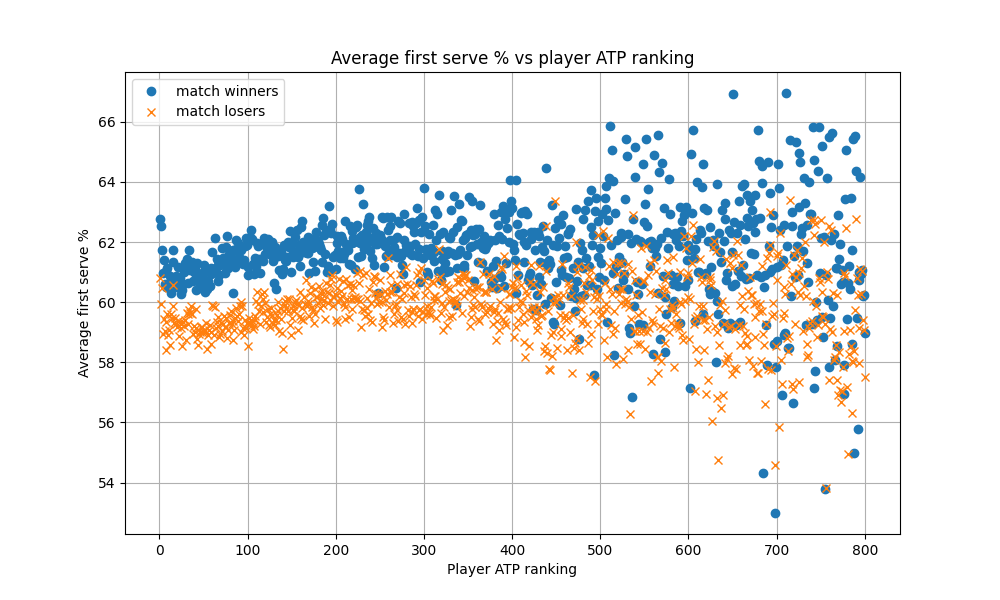
\includegraphics[width=\textwidth]{figures/serve_vs_ranking.png}
    \caption{Znaczenie pierwszego serwisu na różnym poziomie rozgrywek.}
    \label{fig:serve_vs_ranking}
\end{figure}
Pierwszym jasnym wnioskiem jest to, że im większy procent trafionych serwisów, tym większa szansa na zwycięstwo na każdym poziomie rozgrywek. Ciekawą obserwacją jest także to, że najlepsi gracze (top 100) nie trafiają w kort pierwszym serwisem częściej niż gracze z niższych poziomów. Wręcz przeciwnie, średnio trafiają trochę mniej. Może to być związane z tym, że grają przeciwko lepszym zawodnikom, co zmusza ich do podejmowania większego ryzyka i z tym że równie skutecznie potrafią wygrywać punkty po drugim serwisie. Natomiast wyraźna jest różnica w regularności pierwszego serwisu między top 300 a resztą rankingu. Procent trafionych pierwszych serwisów dla pierwszej grupy oscyluje między 58\% a 64\%, dla drugiej grupy jest to między 53\% a 67\%. Wynika z tego, że regularność pierwszego serwisu jest kluczowa, aby wygrywać turnieje i piąć się w rankingu ATP.

Podobne dane mogą być przeanalizowane dla konkretnego zawodnika i jego awansów lub spadków w światowym rankingu. Wykres \ref{fig:serve_Diego} pokazuje jakość pierwszego serwisu stosunkowo niskiego (170 cm) gracza --- Diego Schwartzmana. 
\begin{figure}[h]
    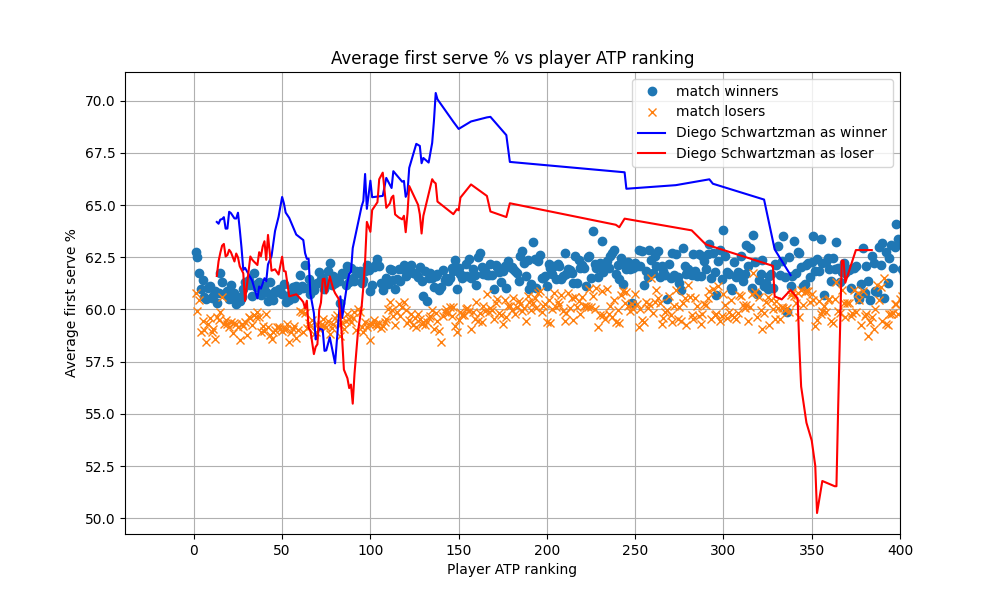
\includegraphics[width=\textwidth]{figures/serve_Diego.png}
    \caption{Pierwszy serwis Diego Schwartzmana na tle innych zawodników na różnym poziomie rozgrywek.}
    \label{fig:serve_Diego}
\end{figure}
Wyraźnie widać, że rankingową wspinaczkę z poziomu 100-300 (turnieje Challenger) do poziomu top 100 (główny cykl ATP --- Wielkie Szlemy i turnieje ATP 1000) Diego zawdzięcza bardzo wysokiej skuteczności pierwszego serwisu (mierzonej jako procent trafionych serwisów). Wysoki procent trafionych pierwszych serwisów może być szczególnie ważny dla niższych zawodników, których drugi serwis bywa słabszy i nie daje znaczącej przewagi przez uwarunkowania fizyczne (uderzanie piłki niżej). Analizując jakość i skuteczność serwisu graczy o podobnych warunkach fizycznych i osiągających sukcesy i monitorując swój własny serwis, rozwijający się gracze mogą zacząć rozwijać to uderzenie w odpowiednim kierunku i odpowiednio zaplanować serwisową strategię, np. zwiększając procent trafionych pierwszych serwisów kosztem siły lub precyzji.


\subsection{Analiza wyników zawodników w zależności od poziomu zmęczenia}
Kondycja fizyczna jest ważnym atrybutem profesjonalnego tenisisty. W typowym turnieju tenisowym (drabinka na 32 graczy), aby wygrać turniej, gracz musi odnieść zwycięstwo w 5 meczach w ciągu paru dni. Wyznacznikiem ilości wysiłku włożonego w mecz (tj. zmęczenia) może być całkowita liczba rozegranych gemów w meczu. W meczu tenisowym do 2 wygranych setów (również nazywane \textit{best of 3}) minimalna liczba rozegranych gemów to 12 (wynik 6-0 6-0), a maksymalna to 39 (wynik 7-6 6-7 7-6). Wykres \ref{fig:win_games_played} przedstawia procent wygranych meczów w drugiej rundzie (R16) typowego turnieju w zależności od liczby rozegranych gemów w rundzie pierwszej (R32).
\begin{figure}[h]
    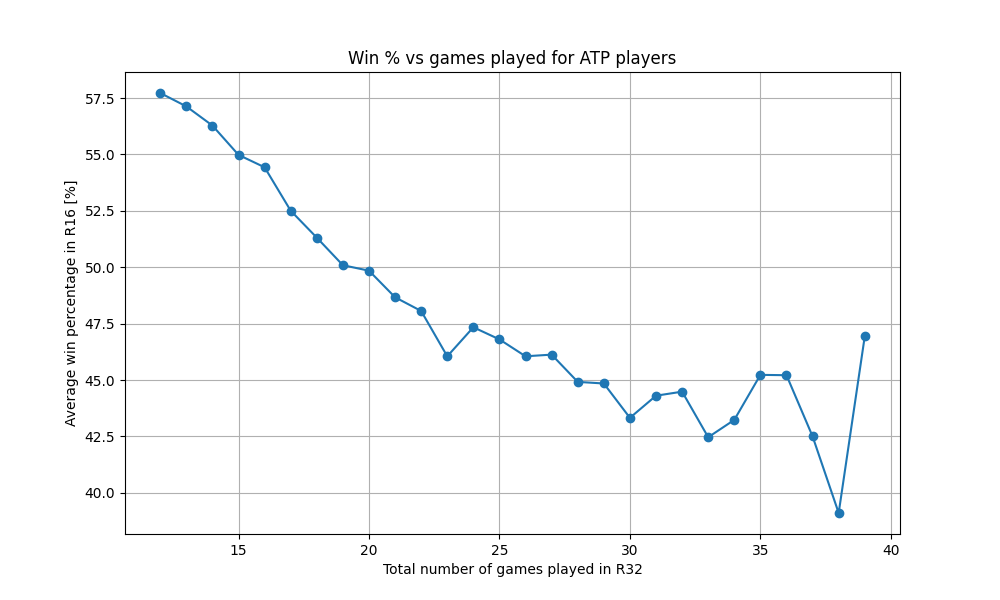
\includegraphics[width=\textwidth]{figures/win_games_played.png}
    \caption{Procent wygranych meczów w drugiej rundzie (R16) w zależności od rozegranych gemów w rundzie pierwszej (R32).}
    \label{fig:win_games_played}
\end{figure}

Jak widać powyżej, zmęczenie znacząco wpływa na wyniki zawodników. Zawodnik, który rozegrał w rundzie pierwszej tylko 12 gemów (wynik 6-0 6-0) ma średnio 57,7\% szans na wygranie drugiej rundy. Natomiast zawodnik, który rozegrał długi 38-gemowy pojedynek pierwszej rundy (np. wynik 7-6 5-7 7-6) ma średnio tylko 39,1\% szans na wygraną w kolejnej rundzie. Równocześnie warto zauważyć, że liczba rozegranych gemów nie jest idealnym miernikiem zmęczenia. Mecze bardzo wysokich graczy posiadających świetny serwis często kończą się wysokim wynikiem (np. 7-6 6-7 7-6) ale niekoniecznie są wyczerpujące fizycznie przez brak długich wymian (piłki są często wygrywane bezpośrednio po serwisie). To może być powodem wahań w procencie wygranych meczów w R16 dla liczby rozegranych gemów w R32 powyżej 30 (widocznych na wykresie \ref{fig:win_games_played}).

Na wykresie \ref{fig:gbr_vs_esp} przedstawiono te same dane, ale z dodatkowym podziałem na pochodzenie zawodników --- przedstawieni są Brytyjczycy (GBR) i Hiszpanie (ESP).
\begin{figure}[h]
    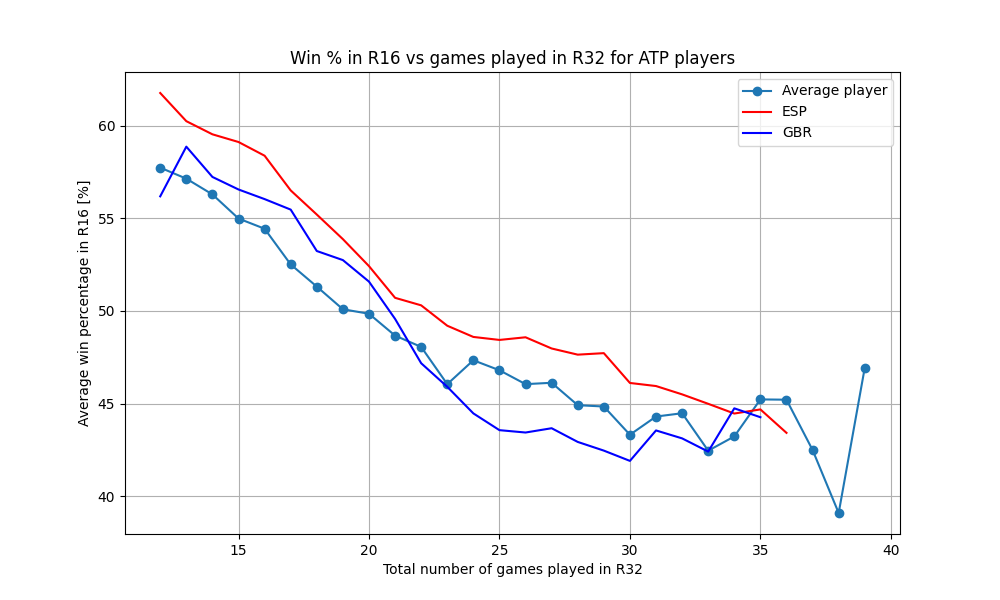
\includegraphics[width=\textwidth]{figures/gbr_vs_esp.png}
    \caption{Porównanie kondycji zawodników brytyjskich (GBR) i hiszpańskich (ESP) na tle średniej.}
    \label{fig:gbr_vs_esp}
\end{figure}
Dla meczów pierwszej rundy, które mogą być uznane za długie i męczące (między 20 a 35 gemów) wyraźnie widać różnicę w procencie wygranych meczów drugiej rundy między Brytyjczykami i Hiszpanami. Co więcej, Brytyjski tenisista wypada również gorzej od średniego gracza. Za przygotowanie fizyczne profesjonalnych tenisistów z Wielkiej Brytanii często odpowiada brytyjski związek tenisowy (LTA). Powyższe dane powinny stanowić podstawę do zmiany brytyjskich treningów kondycyjnych, które mogłyby zostać oparte na modelu hiszpańskim.


\subsection{Analiza skuteczności pierwszego serwisu w zależności od wzrostu zawodnika}
Znaczenie serwisu w tenisie i zależność jego skuteczności od wzrostu zawodnika zostały krótko wspomniane w poprzednich analizach. Wykres \ref{fig:serve_height} pokazuje te zależności, bazując na danych.
\begin{figure}[h]
    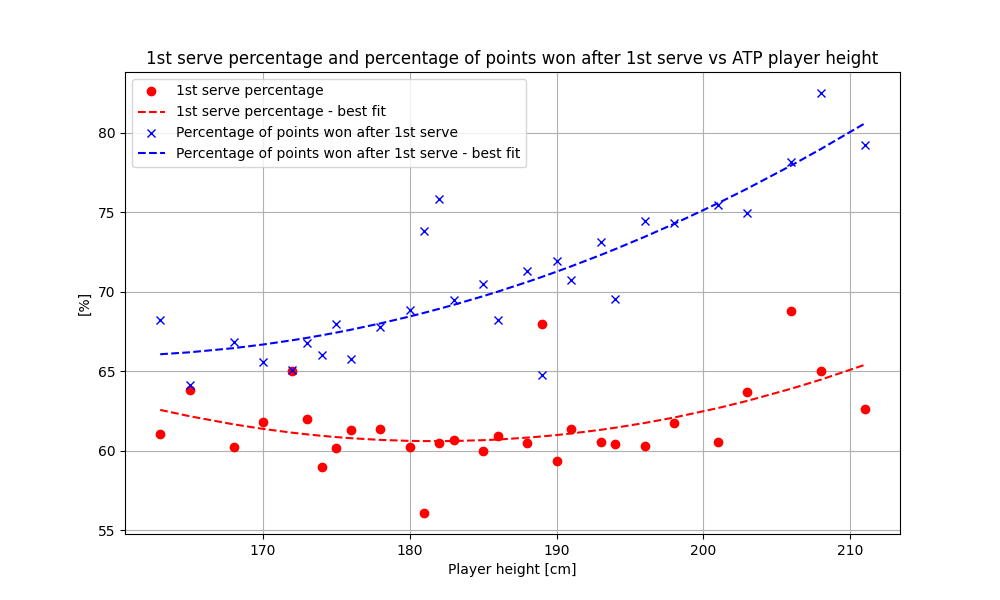
\includegraphics[width=\textwidth]{figures/serve_height.png}
    \caption{Skuteczność pierwszego serwisu w zależności od wzrostu gracza.}
    \label{fig:serve_height}
\end{figure}
Skuteczność pierwszego serwisu wyrażona jest za pomocą dwóch metryk:
\begin{itemize}
    \item Procent trafionych pierwszych serwisów (\textit{1st serve percentage})
    \item Procent wygranych punktów po trafionym pierwszym serwisie (\textit{Percentage of points won after 1st serve})
\end{itemize}
Wyraźnie widać, że trafianie pierwszym serwisem daje przewagę każdemu zawodnikowi (procent wygranych punktów > 64\%) jednak ta przewaga jest zdecydowanie większa dla graczy wyższych. Co ciekawe, procent trafionych pierwszych serwisów jest podobny dla graczy niższych i wyższych. Gracze średniego wzrostu trafiają pierwszym serwisem trochę mniej. Może to być związane z tym, jak warunki fizyczne kształtują styl gry, na przykład:
\begin{itemize}
    \item Gracze niscy częściej trafiają pierwszym serwisem, aby uniknąć słabszego drugiego serwisu, który często jest atakowany.
    \item Gracze wysocy częściej trafiają pierwszym serwisem, aby ograniczyć długość wymian ze względu na gorszą kondycję i mobilność.
    \item Gracze średniego wzrostu (na tle innych tenisistów) są bardziej wszechstronni i mogą sobie pozwolić na większe ryzyko i mniejszy procent trafień przy pierwszym serwisie.
\end{itemize}
Niestety brak bardziej szczegółowych danych w zbiorze danych analizowanym w tym projekcie nie pozwala na sprawdzenie wszystkich powyższych hipotez.

Niemniej jednak rozwijający się gracze powinni monitorować skuteczność swojego serwisu i swojej konkurencji w podobny sposób, aby upewnić się, że to uderzenie jest odpowiednio rozwijane, nie jest gorsze na tle aktualnej opozycji i zapewnia im przewagę w meczach.



\section{Wnioski i zakończenie}
Praca wykazała użyteczność analizy tenisowych danych w celu poprawy przygotowania i wyników zawodnika. Do przetwarzania i analizy danych skutecznie zostały użyte metody, narzędzia i aplikacje do przetwarzania dużych zbiorów danych (\textit{big data}). Użyteczność analizy została wykazana pomimo użycia stosunkowo małego zbioru danych (395,7 MiB) w kontekście big data. Rozszerzenie tego zbioru i przeprowadzenie analiz na większych i bardziej różnorodnych danych (np. historia meczu punkt po punkcie, nagrania wideo meczów, informacje z systemu Hawk-Eye) ma potencjał zrewolucjonizować podejście trenerów, organizacji i samych zawodników do ich tenisowego rozwoju.

\subsection{Ulepszenia i dalsza praca}
Potencjalne ulepszenia tej pracy i dalsza praca do wykonania:
\begin{itemize}
    \item Rozszerzenie zbioru danych o:
    \begin{itemize}
        \item Dane z automatycznej ekstrakcji danych ze stron organizacji ATP i WTA (\textit{web scraping}).
        \item Dane pozyskane z nagrań wideo meczów tenisowych (trajektoria piłki i ruch graczy w każdym punkcie) z użyciem biblioteki OpenCV. Ekstrakcja danych z nagrań wideo mogłaby być również przeprowadzona w czasie rzeczywistym z użyciem takich narzędzi jak YOLOv3 \cite{yolo_v3}.
    \end{itemize}
    Powyższe dane również mogłyby być przerabiane i analizowane za pomocą narzędzi big data.
    \item Użycie AWS Transfer Family to przesyłania plików CSV do S3. Zapewniłoby to solidniejsze i bardziej wszechstronne rozwiązanie w porównaniu z przesyłaniem bezpośrednim (np. zapewniłoby możliwość monitorowania przesyłu). Przysłanie wszystkich plików CSV do S3 zajmowało ponad 20 minut i mogło być podatne na błędy, których AWS Transfer Family pomaga uniknąć. Niestety AWS Transfer Family nie było dostępne w AWS Academy Learner Lab.
    \item Użycie AWS Lambda, aby reagować na nowe commity w repozytorium Jeffa Sackamanna (nowe dane) i automatycznie rozpoczynać cały proces ETL i analizy. AWS Lambda nie było użyte ze względu na ograniczenia czasowe.
    \item Stworzenie dashboardu z dostępem do przetworzonych danych i udostępnienie go trenerom i zawodnikom jako końcowy produkt oparty na danych i komunikacja wyników. Dashboard mógłby być stworzony z użyciem AWS QuickSight (oryginalny plan zakładał użycie tego narzędzia, ale nie było ono dostępne w AWS Academy Learner Lab) lub innego narzędzia do wizualizacji danych i udostępniony w aplikacji webowej. Dashboard pozwalałby na filtrowanie danych, np. wybór zawodnika i przegląd jego statystyk.
    \item Większy zakres oczyszczania danych w procesie ETL. Podczas analizy w EMR Notebook, że więcej danych wymagało oczyszczenia, np. niektóre dane WTA dotyczące pierwszego serwisu były nieprawidłowe (więcej wygranych punktów serwisowych niż zagranych). Podobnie było z danymi dotyczącymi wzrostu zawodniczek WTA.
    \item Większy zakres zastosowania AWS Glue Data Catalog. Poza przeglądaniem informacji o bazie danych zorganizowanych w tabelkach, zastosowanie AWS Glue Data Catalog w tym projekcie było ograniczone. Zalety AWS Glue Data Catalog takie jak przechowywanie scentralizowanych i zorganizowanych metadanych, zapewnienie spójnego interfejsu między narzędziami, czy optymalizacja zapytań mogłyby zostać wykorzystane lepiej przy większej ilości użytych narzędzi AWS.
    \item Uprzątniecie kodu w EMR Notebook. Niektóre fragmenty kodu powtarzały się, ale miały różne parametry. Mogłyby zostać zastąpione funkcjami.
    \item Poza tenisem męskim (ATP), dodatkowe przeanalizowanie podobnych zależności w profesjonalnym tenisie żeńskim (WTA). Jakość dostępnych danych WTA była nieco gorsza niż danych ATP.
    \item Automatyczne testowanie kodu (\textit{unit testing}).
\end{itemize}



% \nocite{*} % This line includes all references in the bibliography
\renewcommand{\refname}{Bibliografia}
\addcontentsline{toc}{section}{\refname}
\bibliographystyle{IEEEtran}
\bibliography{bibliography/references}


\begin{appendices}
\renewcommand{\appendixname}{Załącznik}

\section{Opis surowych danych} \label{sec:raw_data_description}
Oryginalny opis poszczególnych kolumn w plikach CSV dostępny jest w jednym z repozytoriów Jeffa Sackmanna \cite{tennis_atp} pod tym linkiem:
\href{https://github.com/JeffSackmann/tennis_atp/blob/master/matches_data_dictionary.txt}{LINK}

Kolumny w surowych plikach CSV ze statystykami meczów, których dane zostały użyte w tym projekcie, opisane są poniżej:
\begin{itemize}
    \item \verb|tourney_id|: unikalny identyfikator turnieju tenisowego.
    \item \verb|surface|: nawierzchnia kortu, na której został rozegrany mecz.
    \item \verb|winner_id|: unikalny identyfikator gracza, który wygrał mecz.
    \item \verb|winner_name|: imię i nazwisko gracza, który wygrał mecz.
    \item \verb|winner_ht|: wzrost gracza, który wygrał mecz.
    \item \verb|winner_ioc|: narodowość gracza, który wygrał mecz.
    \item \verb|loser_id|: unikalny identyfikator gracza, który przegrał mecz.
    \item \verb|loser_name|: imię i nazwisko gracza, który przegrał mecz.
    \item \verb|loser_ht|: wzrost gracza, który przegrał mecz.
    \item \verb|loser_ioc|: narodowość gracza, który przegrał mecz.
    \item \verb|score|: wynik meczu zapisany jako tekst (np. ,,6-3 1-6 7-5'').
    \item \verb|best_of|: format meczu (maksymalnie 3 sety lub maksymalnie 5 setów).
    \item \verb|round|: turniejowa runda, w której został rozegrany mecz.
    \item \verb|w_svpt|: liczba punktów serwisowych gracza, który wygrał mecz.
    \item \verb|w_1stIn|: liczba trafionych pierwszych serwisów przez gracza, który wygrał mecz.
    \item \verb|w_1stWon|: liczba punktów wygranych po trafionym pierwszym serwisie przez gracza, który wygrał mecz.
    \item \verb|l_svpt|: liczba punktów serwisowych gracza, który przegrał mecz.
    \item \verb|l_1stIn|: liczba trafionych pierwszych serwisów przez gracza, który przegrał mecz.
    \item \verb|l_1stWon|: liczba punktów wygranych po trafionym pierwszym serwisie przez gracza, który przegrał mecz.
\end{itemize}
\end{appendices}


\end{document}
